% IEEE standard conference template; to be used with:
%   spconf.sty  - LaTeX style file, and
%   IEEEbib.bst - IEEE bibliography style file.
% --------------------------------------------------------------------------

\documentclass[letterpaper]{article}
\usepackage{spconf,amsmath,amssymb,graphicx,float, graphicx}

% Example definitions.
% --------------------
% nice symbols for real and complex numbers
\newcommand{\R}[0]{\mathbb{R}}
\newcommand{\C}[0]{\mathbb{C}}

% bold paragraph titles
\newcommand{\mypar}[1]{{\bf #1.}}

% Title.
% ------
\title{Acceleration of Large Displacement Optical Flow Estimation}
%
% Single address.
% ---------------
\name{Saiwen Wang, Yifan Su, Yijun Pan, Xinyuan Yu} 
\address{Department of Computer Science\\ ETH Z\"urich\\Z\"urich, Switzerland}

% For example:
% ------------
%\address{School\\
%    Department\\
%    Address}
%
% Two addresses (uncomment and modify for two-address case).
% ----------------------------------------------------------
%\twoauthors
%  {A. Author-one, B. Author-two\sthanks{Thanks to XYZ agency for funding.}}
%    {School A-B\\
%    Department A-B\\
%    Address A-B}
%  {C. Author-three, D. Author-four\sthanks{The fourth author performed the work
%    while at ...}}
%    {School C-D\\
%    Department C-D\\
%    Address C-D}
%

\begin{document}
%\ninept
%
\maketitle
%

\begin{abstract}

DeepFlow \cite{Weinzaepfel:2013:DLD:2586117.2586991} is a state-of-the-art flow estimation algorithm which 
computes the relative displacement of pixels in a pair of images. Despite the theoretical bound of the algorithm, achieving high performance at the implementation stage proves to be a non-trivial task. In order to solve the dense non-linear system efficiently, certain optimisation for modern processors like unrolling can be applied. We further experimented with locality enhancement and vectorisation which help achieve marginal improvement over a standard implementation.  
\end{abstract}

\section{Introduction}\label{sec:intro}

Nowadays, many computer vision systems utilise optical flow detection as an early stage of the pipeline. Cases of small displacement has been extensively studied over the past few decades. That is, the motion of every pixel is limited to a few pixels. Cases of unconstrained motion have received attention only recently and it remains an open problem \cite{Brox:2011:LDO:1936329.1936562, 5539820}. Large displacement optical flow covers the more realistic cases where the motion is not restricted and can be larger than the size of the object. The typical result of optical flow estimation is shown in Figure 1.
\begin{figure}[H]\centering
  \includegraphics[scale=0.25]{intro.eps}
  \caption{Result of Optical Flow. (a)Two original overlapped images; (b) Real displacement of the two; (c) Vector representation of the displacement result found by optical flow; (d)Displacement result found by optical flow.}
\end{figure}

\mypar{Motivation}
An enormous amount of visual content from different sources (e.g. wearable devices) is becoming available, along with new challenges like visual-based localization from realistic videos which further put an emphasis on processing speed. State-of-the-art optical flow algorithm provides a solid theoretical base for the estimation problem. But standard implementations usually work inefficiently on large datasets due to the complexity of updating and solving a dense non-linear system within multiple iterations. In our work, we experimented with several optimization methods and present an implementation which is marginally faster than the unaccelerated version.

\mypar{Related work} 
Many state-of-the-art optical flow estimation algorithms work in the framework of variational method. Horn and Schunck \cite{Baker:2004:LYU:964568.964604} introduced a classical way of minimising an energy function based on a data term and a smoothness term. Ever since, research has focused on alleviating the drawbacks of this method. A series of improvements were proposed over the years. Brox and Malik \cite{Brox:2011:LDO:1936329.1936562} propose to add a matching term penalising the difference between flow estimation and matches. Xu\cite{5539820} performs an expensive fusion of intensity flow, SIFT feature matches \cite{Szeliski}  and patch matches \cite{Barnes:2010:GPC:1927006.1927010} at each level of image pyramid. DeepFlow \cite{Weinzaepfel:2013:DLD:2586117.2586991} blends a matching term into the energy function and proposes a global matching algorithm, tailored to the optical flow problem, that allows to alleviate the over-constrained smooth terms on fast motions.\\
Our method improves time and memory efficiency based on DeepFlow's energy function and utilises several modern optimization technology, including blocking and instruction-level parallelism. The experiment result shows an effective  acceleration of the implementation.

\section{Background}\label{sec:background}

In this section, we formally define the energy function of used in Deepflow \cite{Weinzaepfel:2013:DLD:2586117.2586991}, highlight some details of the algorithm and perform a cost analysis.

\mypar{Energy Function of DeepFlow}
Deepflow is one of the optical flow estimation algorithm based on variational method, and it introduces pre-calculated keypoint matches into the energy minimization framework. The baseline for such an optical flow estimation method is to minimise an energy function constituted of a data term, a smoothness term and a matching term. 
\begin{equation}
  E(\omega) = \int_{\Omega}^{} E_{D} + \alpha E_{S} + \beta E_{M} {\rm d}x
\end{equation}
The first term typically assumes that the colour and the gradient are constant along the flow while the second term enforces the local smoothness of the estimation. A matching term to penalise the difference between the input matches and the estimated flow is added to the classic data and smoothness terms. A concrete definition of the three terms is as below. Detailed derivation can be referred to \cite{Weinzaepfel:2013:DLD:2586117.2586991}.
\begin{equation}
  E_{D} = \delta \psi(\sum_{i=1}^{c}\omega ^{T}\overline{J}_{0}^{i}\omega) + \gamma \psi(\sum_{i=1}^{c}\omega ^{T}\overline{J}_{xy}^{i}\omega)
\end{equation}
\begin{equation}
  E_{S} = \psi (\left \| \bigtriangledown u \right \|^{2} + \left \| \bigtriangledown v \right \|^{2})
\end{equation}
\begin{equation}
  E_{M} = c\Phi \psi (\left \| w-w^{'} \right \|^{2})
\end{equation}
The algorithm flow is then drawn as Figure 2.
\begin{figure}[H]\centering
  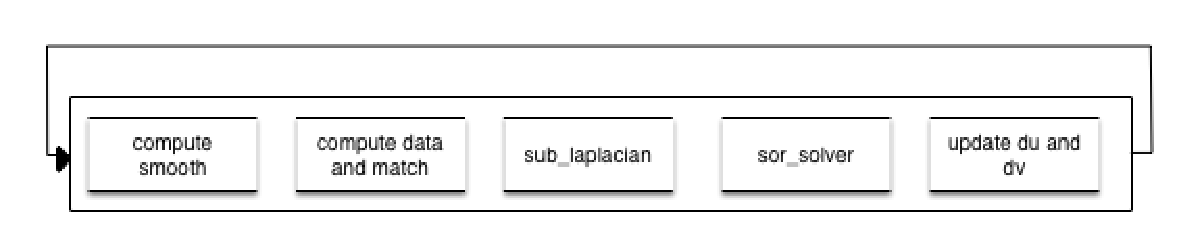
\includegraphics[scale=0.41]{flow.eps}
  \caption{Algorithm Flow of One Iteration.}
\end{figure}
The energy function is then minimized through a coarse-to-fine scheme within a multi-scale image pyramid. The flow estimated at a coarse level of the image pyramid is further used as initialisation at the consecutive level. First part of each iteration computes the above three terms. It is then optimised using fixed point iterations and classic linear system solver such as SOR(Successive Over Relaxation).

\mypar{Cost Analysis}
For cost analysis, we measure flops as (addition, multiply, division, square root). We count each type of operation for simplicity. In fact, divisions and sqrts both cost 28 cycles. Regarding them as one flop may underestimate flop count, which leads to lower performance.\\
The cost of solver function is $41MNK_iK_mK_o$ flops with M, N as the height and the width of the input image, $K_i$, $K_m$, $K_o$ as the numbers of inner, middle and outer loops. The compute function costs $263MNK_mK_o$ flops.\\
The time and memory complexity of the two functions we optimised is shown in Table 1, where m = width of  input image(pixel), n = height of input image(pixel), $K_{pyr}$ = pyramid level of each iteration, $K_{inner}$ = inner loop of each iteration, $K_{solver}$ = inside loop of solver function.
\begin{table}[h]\centering
\footnotesize
\begin{tabular}{|l|l|l|l|l|}
\hline
 Function & Time/Memory Complexity\\ \hline
 Sor Solver & $O(K_{pyr} * m * n * K_{inner}* K_{solver})$ \\ \hline
 Compute Data and Match & $O(K_{pyr} * m * n * K_{inner})$ \\ \hline
\end{tabular}
\caption{Time \& Memory Complexity}
\end{table}

\section{Method}\label{sec:method}

In this section we will present our step-wise implementation of the 
algorithm and indicate detail optimization methods. 

\mypar{Baseline}
The baseline implementation of the algorithm is given by the authors 
of the paper \cite{Weinzaepfel:2013:DLD:2586117.2586991}. It's 
implemented in a naive manner and no optimization method is performed. 

The core algorithm subsamples the pair of original input images into 
a stack of different size of images, which looks very similar to the 
pyramid. For each pair corresponding subsampled images in the 
pyramid, both the first and second order derivative is computed and 
the flow will be computed in iterations. In each of the iteration, 
The smoothing term will be first computed and then served to the 
matching computation. After that a linear system will be solved and 
after each iteration the offset (displacement) will be updated. 

All these algorithm will first go through the smallest image in the 
pyramid, and then the computed displacement of the previous images 
in the pyramid will become a base which helps to compute the displacement 
of the next image. In the end, the displacement of the original image 
will be computed and the algorithm terminated. 

\mypar{Bottleneck}
After implementing the baseline version of the algorithm, we tried to 
analyze the performance bottleneck. By using google profiler, the plot 
of the calling graph below can be helpful to find the performance 
hotspot. 

It's obvious that the majority of the time is consumed by function 
\texttt{sor\_solver} and \texttt{compute\_data\_and\_match}. So in the 
following part of the optimization steps, we will focus in optimizing 
these two functions. 



\mypar{Basic Optimizations}
We first apply some basic optimization methods to the code. 

\emph{Code motion.} We observe some repeated division sub-expressions 
in the code. It is known that division operations has lower throughput 
and requires longer cycles to finish computation. By replacing division
sub-expressions with precomputed shared values, the number of computation 
flops is expected to be lower. 

\emph{Scalar replacement. } We observed that the code requires large 
amount of memory access. The original image and sub-sampled images,  
helper values includes first and second order derivative and displacement 
results are all stored in memory. In each inner iteration, multiply 
values in the memory are accessed multiple times. We apply scalar 
replacement to memory location being accessed. Thus repeated memory 
accesses are reduced to two (one for loading and one for storing). 

\begin{figure}[H]\centering
  \includegraphics[scale=0.35]{bottleneck.eps}
  \caption{Bottleneck of Algorithm Flow. Time consumption percentage 
  is showed in each function box. }
\end{figure}
\mypar{Memory and locality}
\emph{Reuse memory. } As indicated above, the algorithm requires large 
amount of memory. It is noticeable that for each single (possible sub-sampled) 
image, 23 helper data structures with the same size of the image will be 
created and accessed. The large amount of momory space is too large 
to be fitted in either the first level cache or the second level. 

In order to reduced the possible data transfer between cache and 
memory, we try to reduce the number of the duplicated helper data 
structures. We decide to use a unique set of helper data structure 
for all size of sub-sampled images, instead of creating a different 
set for each of sub-sampled images. 

After the reuse of memory, we expect the memory of the helper data structure 
is already sitted in the cache when revisiting them in the next iteration, 
which introduce temporal locality. 

\emph{Unrolling.} In each of the inner iteration, the data of input image 
and helper data structure is accessed one by one in a row order. For 
the solver part, not only the corresponding pixel is access, the nearby 
pixels (the upper, lower, left and right, which form like a cross) are also 
accessed. We observed a strong spatial locality here. 

As indicated above, the large number of helper structures and possible 
data alignment can cause repeated cache misses when accessing neighbour 
pixel even if strong spatial locality is observed. We use unrolling the 
increase the spatial locality and try to load as much as possible in 
each transferred cache block and separate the memory access and computation. 

For function \texttt{compute\_data\_and\_match}, only the corresponding 
pixel is accessed and there's no dependence between each pixel. So 
basic unrolling is performed and 16 pixel of \texttt{float} data is loaded 
from every helper structure, computed and then written back. 

For function \texttt{sor\_solver}, accessed pixels are not only neighbour 
pixels in the same row, but also some pixels in the upper and lower row. 
So the unrolling is done by blocking, which introduce blocking size of 
either 2 by 2 or 4 by 4. So the expected memory access can be reduced 
as the data in each cache block can be accessed at once instead of 
possibly repeated access and transferred. 


\mypar{Vectorization}
In the code we observed that same computation is done pixel by pixel in 
the inner iteration. So vectorization is a good possible way to speed 
up computation. 

First we change the compiler flag to enable automatically vectorization. 
And then we introduce intel AVX \cite{firasta2008intel} intrinsic to 
manually performs vectorization. Neither the input images nor the 
sub-sampled image promise row alignment of 8 \texttt{float}. We add 
build-in row alignment of 8 so that all the images are forced to have 
row length divisible by 8. 

In function \texttt{sor\_solver}, neighbour pixel computations are 
correlated, so AVX is not performed on the major part if the code, but 
only to the part of matrix operation. 

\section{Experimental Results}\label{sec:exp}

In the experiment part, we show the performance plots and roofline model of the optimized algorithm.

\mypar{Experimental setup} We setup experiment on a machine with Sandy Bridge processor. The compiler is gcc with version 4.9.2 on Redhat Linux. We use \texttt{-O0} and \texttt{-fno\allowbreak-tree-vectorize} as compiler flag firstly and then change it to \texttt{-03} and \texttt{-core-avx-i} in the latter experiment. The input of our program is a pair of images with slight difference. In our experiment, we test with images in a range from  26 $\times$ 64 to 4096 $\times$1716

\mypar{Results}
Since we optimize two functions in the algorithm, we show the results of each optimized function separately.

\begin{figure}[H]\centering
  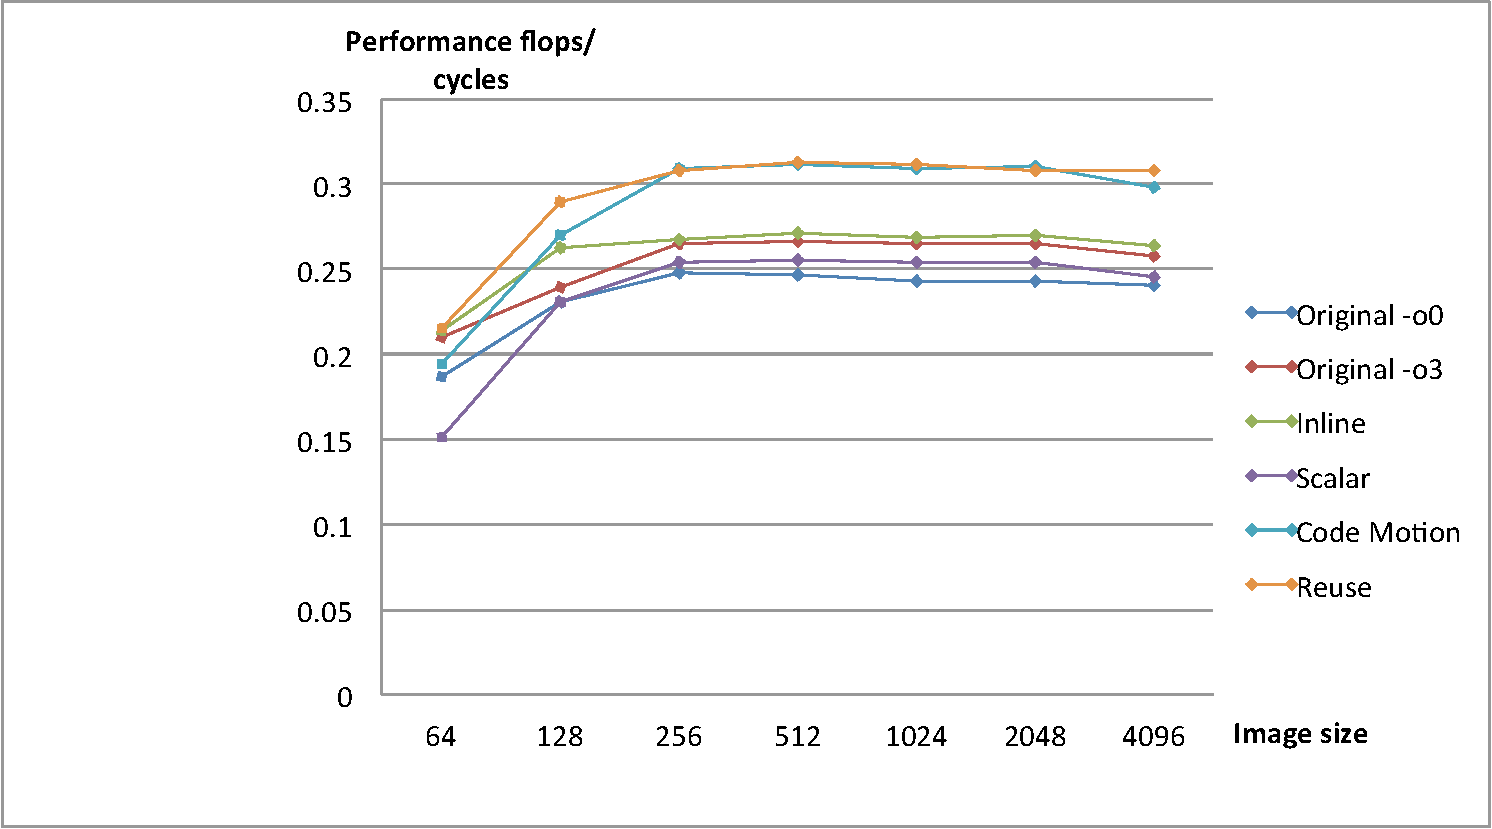
\includegraphics[scale=0.33]{compute_no_avx.pdf}
  \caption{performance plot of Compute Data and Match without AVX}
\end{figure}
Fig 4. is the performance plot of Compute Data and Match without AVX. We can see the performance is improved slightly after scalar replacement and code motion. In Scalar replacement part, we reduce duplicate memory access. In the code motion part, we precompute share division components, which is very expensive. Then, we change the compiler flag to -O3 and -core-avx-i which improves the performance by 25\%.
\begin{figure}[H]\centering
  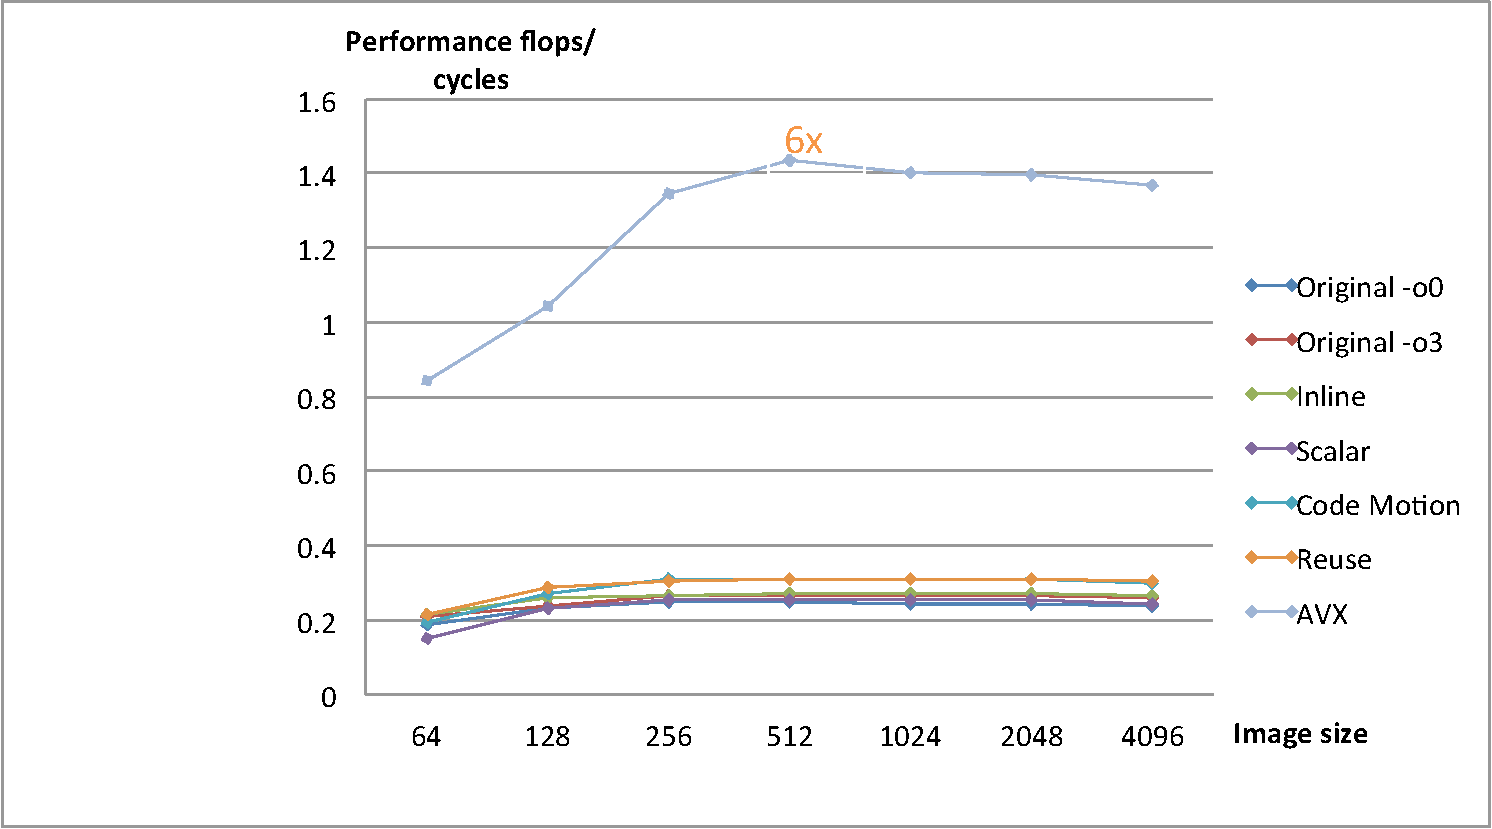
\includegraphics[scale=0.33]{compute_with_avx.pdf}
  \caption{performance plot of Compute Data and Match with AVX}
\end{figure} 

In Fig 5. we can see that the code benefits from blocking and parallel computing by using AVX. The performance is improved significantly. Since we test on a Sandy Bridge machine, the peak performance is 16 flops/cycle. The final performance we get is 1.4 flops/cycle, which is 6 times of the performance of the original code. It is about 8.8\% of the peak performance.

\begin{figure}[H]\centering
  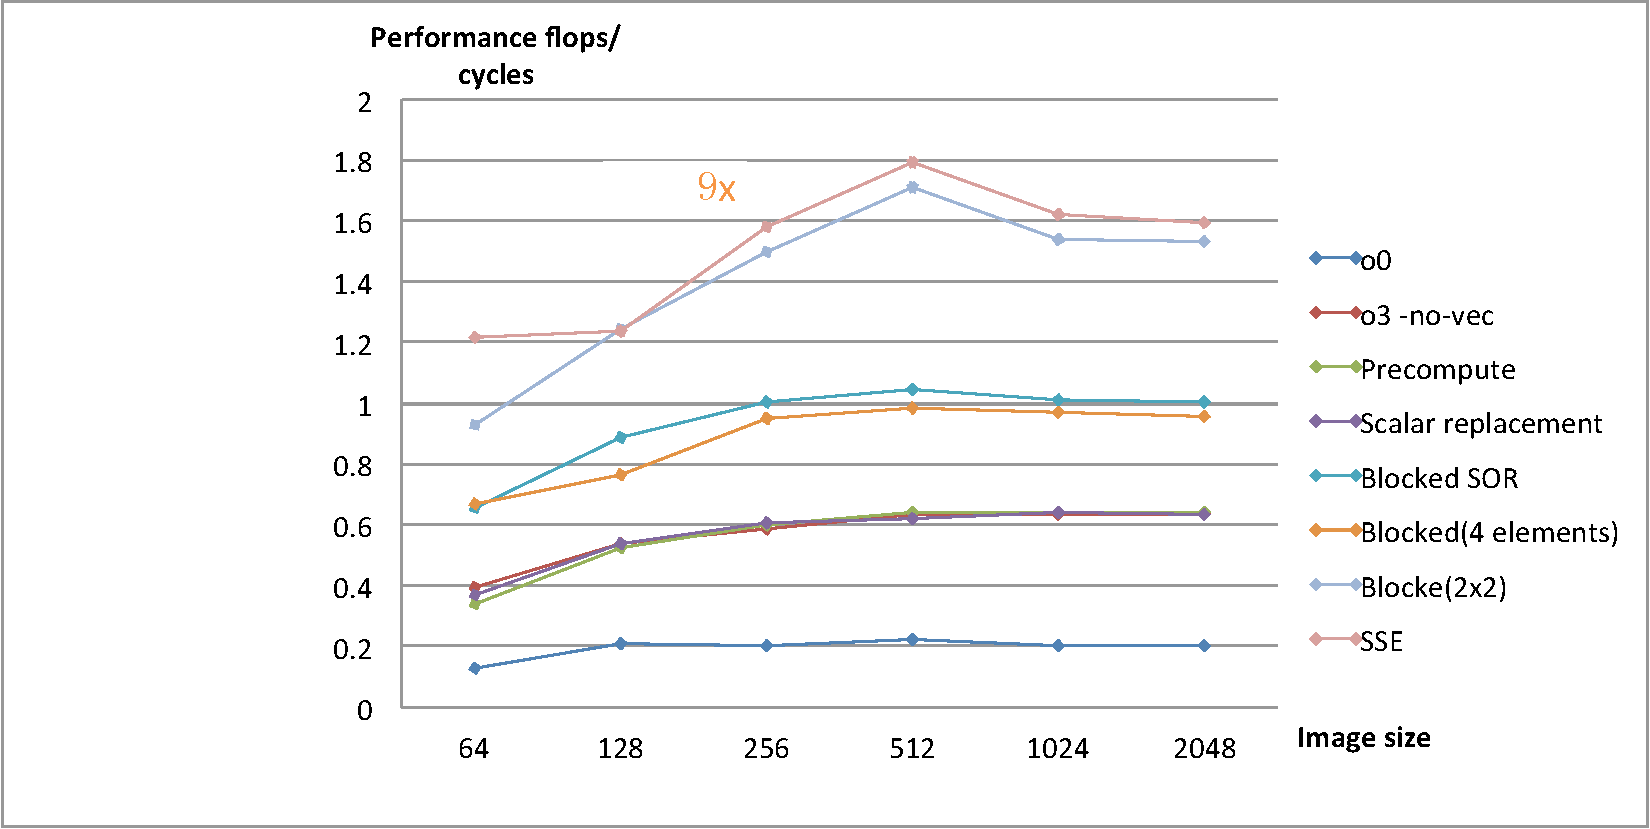
\includegraphics[scale=0.3]{solver.pdf}
  \caption{performance plot of solver}
\end{figure}

In Fig 6. we can see that there are three optimizations which improve the performance significantly, which are changing compiler flag from -o0 and -fno-tree-vectorize to -o3, blocking and blocking with 2 $\times$ 2 mini block.

The code can benefit from better locality by using mini blocks with the size of 2 $\times$ 2. However, in the function of solver, only a little part can be changed to SSE. Thus the performance is not improved much by the optimization of SSE.
In this way, it is meaningless to optimize the function using AVX as well.

In the part of solver function, the performance is improved to 1.8 flops/cycle, which is 9 times of the original performance(0.2 flops/cycle).
Since the peak performance of Sandy Bridge is 8 flops/cycle with SSE. Thus, it is 22.5\% of the peak performance.

\begin{figure}[H]\centering
  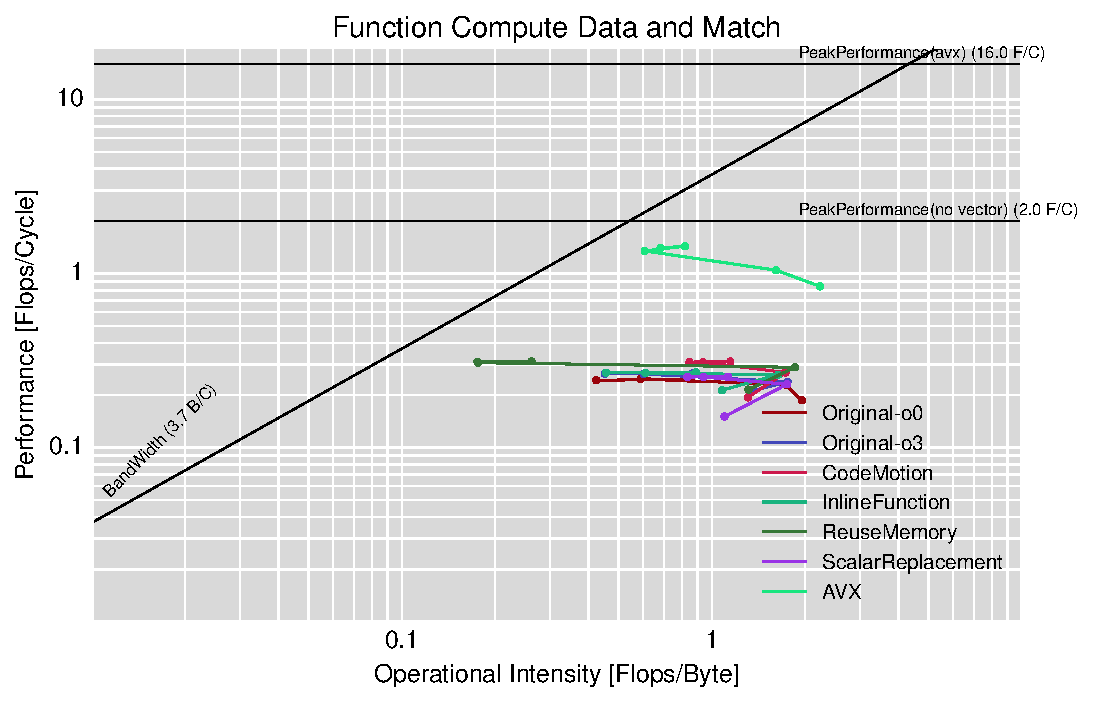
\includegraphics[scale=0.45]{roofline_compute.pdf}
  \caption{roofline of compute data and match}
\end{figure}

Fig 7 is the roofline model of compute data and match function. In the roofline model, we can see that the intensity is affected by the size of input image. If small image is used, most of data can be saved in cache. We have less data transfer and the intensity is higher than using large image. Besides, in our algorithm, there are several division and SQRT operations, which are expensive. If we re-weight one division or SQRT operation by 16 flops (a div or SQRT operation costs 16 cycles while mul costs only 1 cycle), the performance is close to peak performance. Therefore, our algorithm is computational bound.


\begin{figure}[H]\centering
  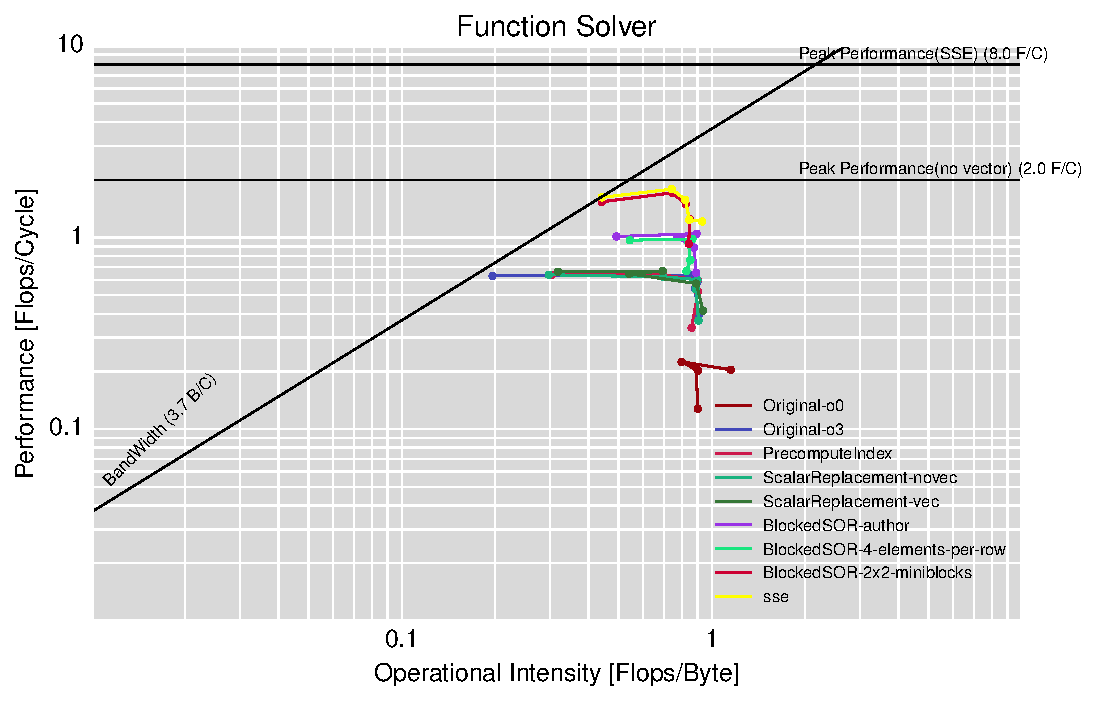
\includegraphics[scale=0.45]{roofline_solver.pdf}
  \caption{roofline of solver}
\end{figure}  

Fig 8 is the roofline model of function of solver. In this model, after re-weighting the division operation, the performance is close to the peak performance. Although, when using large image size, the point is close to the memory bound, we can see the performance is not affected. Thus, we can conclude that the performance is not affected by memory transfer. It is also computational bound in this part.

\section{Conclusions}

By applying our optimization methods to the baseline implementation, significant increase of performance has been achieved. We have gained up to 5.6 and 7 time speedup in the two major bottleneck functions. While the other parts of the algorithm contribute only a small portion to the computation time and no overhead is introduced by our optimisation, the overall 
performance of the Deepflow algorithm also receives noteworthy improvement. 

Our optimization of the Deepflow algorithm can be useful to any 
application which requires intensive optical flow computation. 
The key optimisation techniques can also be applied to similar image 
processing algorithms. 

In future work, we expect to continue minimizing memory footprint of our 
algorithm. An approximation schedule to the origin algorithm which alleviates the strong dependency between neighbour pixels in the multi-stage solver will most likely further reduce the computation time. 

% References should be produced using the bibtex program from suitable
% BiBTeX files (here: bibl_conf). The IEEEbib.bst bibliography
% style file from IEEE produces unsorted bibliography list.
% -------------------------------------------------------------------------
\bibliographystyle{IEEEbib}
\bibliography{bibl_conf}

\end{document}
